\documentclass[titlepage,landscape]{seminar}
\usepackage{url}
\usepackage{graphicx}
\usepackage[pdftex]{color}
\usepackage{hyperref}
\usepackage{epstopdf}
\usepackage{slides}

\newcommand{\frack}{\frac{1}{k}}
\newcommand{\quarter}{\frac{1}{4}}

\begin{document}

\myslide{
\begin{center}
\resizebox{\textwidth}{!}{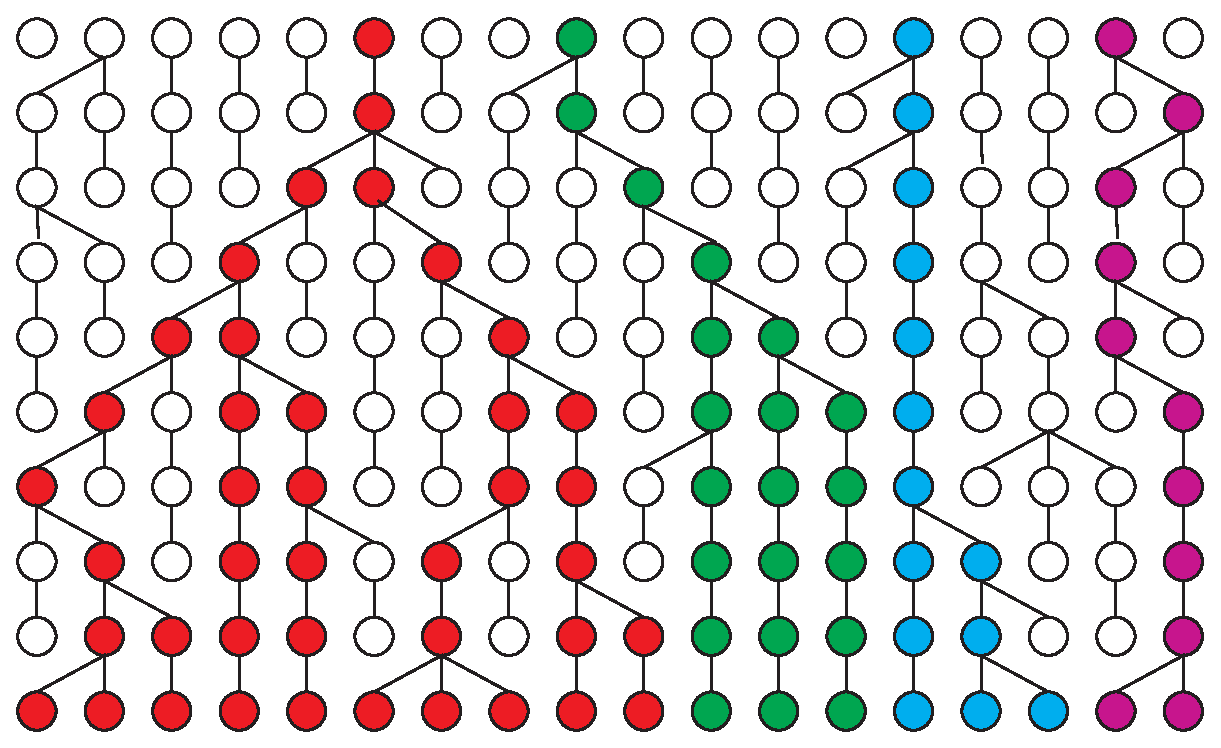
\includegraphics{coalescent-figure.eps}}
\end{center}
}

\myslide{
\heading{Kingman's coalescent (two allele copies)}

\[
\mbox{P}(\hbox{two alleles ibd}) = \frac{1}{2N_e^{(f)}}
\]
\vfill
\[
\mbox{P}(\hbox{coalescent at time $t$} = \left(1 - \frac{1}{2N_e}\right)^{t-1}\frac{1}{2N_e}
\]
\vfill
\[
\hbox{Average time to coalescence of two alleles} = 2N_e
\]
}

\myslide{
\heading{Kingman's coalescent (multiple allele copies)}

\begin{eqnarray*}
m &=& \hbox{number of allele copies} \\
\hbox{number of allele copy pairs} &=& \frac{m(m-1)}{2} \\
\mbox{P}(\hbox{coalescent involving one pair of alleles}) &=& 
\left(\frac{m(m-1)}{2}\right)\left(\frac{1}{2N_e}\right) \\
\hbox{Average time to coalescent event} &=&
\left(\frac{2}{m(m-1)}\right)\left(2N_e\right) \\
&=& \frac{4N_e}{m(m-1)} 
\end{eqnarray*}
}

\myslide{
\heading{Kingman's coalescent (multiple allele copies)}

\begin{eqnarray*}
\hbox{Average time to coalescent event} &=& \frac{4N_e}{m(m-1)} 
\end{eqnarray*}
Now there are $m-1$ alleles
\begin{eqnarray*}
\hbox{Average time to next coalescent event} &=& \frac{4N_e}{(m-1)(m-2)} 
\end{eqnarray*}
\vfill
\begin{eqnarray*}
\bar t &=& \sum_{k=2}^m \frac{4N_e}{k(k-1)} \\
       && \mbox{TAMO} \\
       &=& 4N_e\left(1 - \frac{1}{m}\right) \\
       &\approx& 4N_e
\end{eqnarray*}
}

\myslide{
\heading{Mitochondrial Eve}

Data
\begin{itemize}

\item Mitochondrial DNA from 147 humans

\item Most recent common ancestor 200,000 years ago

\end{itemize}

Expectation
\begin{itemize}

\item All mitochondrial genomes share a single common ancestor $2N_e$
  generations ago.

\item Human generation time $\approx$ 20 years. 

\item 200,000 years $\approx$ 10,000 generations.

\item Coalescence of all mitochondria consistent with $N_e$ of 5000.

\end{itemize}
}

\myslide{
\heading{Coalescent in structured populations}

{\small
\begin{eqnarray*}
\bar t_0 &=& \mbox{average time to coalescence of allele copies from
             the same population} \\
\bar t_1 &=& \mbox{average time to coalescence of allele copies from
             different populations} \\
\bar t &=& \mbox{average time to coalescence of allele copies} \\
       &=& \frac{k(k-1)\bar t_1 + k\bar t_0}{k^2}
\end{eqnarray*}
}
\vfill
If mutation is rare,
\[
F_{st} = \frac{\bar t - \bar t_0}{\bar t} \quad .
\]
}

\end{document}

